\RequirePackage[l2tabu, orthodox]{nag} % generates warnings for stuff you shouldn't do
\documentclass[conference, a4paper]{IEEEtran}

\usepackage[utf8]{inputenc}
\usepackage{lipsum} % dummy text
%\usepackage{multirow} % Allows for multiple rows
%\usepackage{multicol} % Allows for multiple columns
\usepackage{pdflscape} % rotate pages (used for the table) 
\usepackage{rotating}

% Table preamble
\usepackage{xtab, array, booktabs, ragged2e, pdflscape}
\usepackage{changepage}
\usepackage[showframe=true]{geometry}
\PassOptionsToPackage{hyphens}{url}\usepackage[hidelinks]{hyperref}	% Breaks URLs down and allows the document to link to sections

% Bibliography preamble
\usepackage[style=apa,backend=biber,sorting=none]{biblatex}	% APA style biblatex
\addbibresource{references.bib}		% Path of the library

% Images preamble
\usepackage{graphicx}				% Import graphics
% \graphicspath{ {./img/} }	        % Set path to images
\usepackage{wrapfig}			    % Wrap figure around text
\usepackage{tikz}				    % Draw shapes
\usetikzlibrary{positioning,chains} % Libraries used by Tikz
\usepackage{float}					% Correcting the positioning of images
%\usepackage{adjustbox}				% Wrapper for images
%\usepackage[labelfont=bf]{caption}	% Caption generated text
%\usepackage{subcaption}				% Allow sub captions


\title{Automatic Detection of Mind Wandering from Multimodal Datastreams:\\ 
A Survey of State-of-the-art Methods}
%\author{Murtadha Al Nahadi, Robin Faber, Justin de Haan, Wessel Turk}

\author{\IEEEauthorblockN{Murtadha Al Nahadi, Robin Faber, Justin de Haan and Wessel Turk}
\IEEEauthorblockA{Delft University of Technology\\
Delft, Netherlands\\
\{M.AlNahadi, R.J.Faber, J.C.deHaan, W.R.A.Turk\}@student.tudelft.nl}}
\date{March 2019}


\begin{document}
\maketitle
\begin{abstract}
    This document is a model and instructions for \LaTeX.
    This and the IEEEtran.cls file define the components of your paper [title, text, heads, etc.]. *CRITICAL: Do Not Use Symbols, Special Characters, Footnotes, 
    or Math in Paper Title or Abstract.
    \end{abstract}
    
    \begin{IEEEkeywords}
    component, formatting, style, styling, insert
    \end{IEEEkeywords}


\section{Introduction}
Mind wandering (MW) is a phenomenon where the thoughts of a person shift from task-related to task-unrelated for a certain period of time.
Every person has probably experienced it at some point and it can come paired with inefficiency and distraction. 
In situations where attention is needed, such as driving, it is important that the mind wanders as little as possible so people can focus on the task at hand. 
Recent research has clearly shown that inattention when driving has an indisputable impact on road safety \cite{berthie2015restless}. 
It is clear that automated detection and prevention of mind wandering in such settings could be a good solution to the problem. 

This study aims to identify possible challenges in the field of automatic detection of MW in order to further develop it or to be used as a starting point for people who wish to do research and want an overview of the possibilities and what has been done already. This goal is accomplished by giving a structured overview of the state-of-the-art methods in the field and reasoning about the broader context of these studies.

We investigated the following aspects of existing research:
In which tasks is the automatic detection of MW being utilized? Which modalities are used? Which sensors are used for recording these modalities and which features are extracted from them? How is MW being reported by the participants? Which machine learning (ML) algorithms are used to train the model and what performance is achieved by the model? In which environment has the data been collected and has this data been made publicly available? 


\section{Definition of Mind Wandering}

\section{Detection of Mind Wandering}

\section{Methodology}

In order to identify all articles that may be deemed relevant, a highly systematic approach was used that can be broken down into six steps (Fig. \ref{fig:prisma}).

First, 10 articles were hand-picked that were identified as relevant for our goal. These hand-picked articles served as a baseline for the upcoming search of online libraries.
A systematic search on Scopus and Web of Science was performed to identify all articles aimed at the detection of mind wandering. The retrieved articles were checked on relevancy and completeness.
An indication of the completeness of the search terms used was obtained by comparing the results of the online libraries with the baseline. 
The used search terms were tweaked by making them broader when the results contained a low number of articles and few baseline articles and made narrower when there were many irrelevant articles retrieved.
A logbook of the used search terms can be found in Appendix A.
As a result of this first step, an initial list of 125 articles was obtained.

\begin{figure}
  \resizebox{\columnwidth}{!}{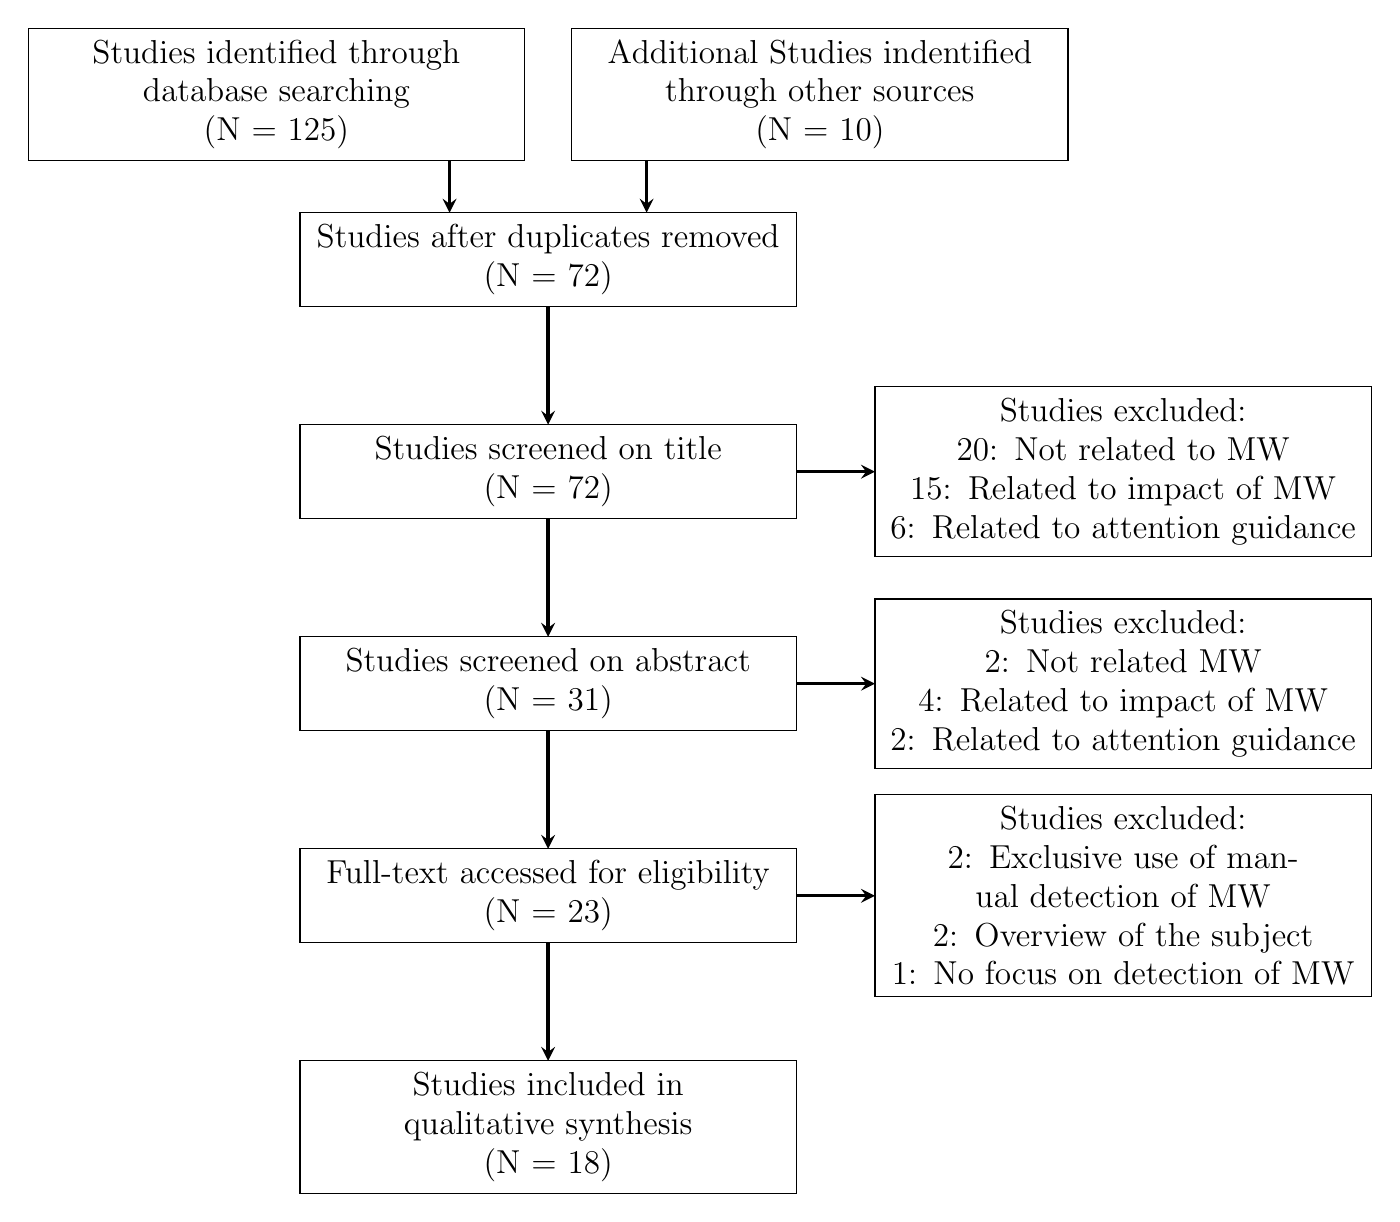
\begin{tikzpicture}[
    node distance=15mm and 10mm,
    start chain=going below,
 mynode/.style = {
        draw, rectangle, align=center, text width=60mm,
        font=\large, inner sep=1ex, outer sep=0pt,
        on chain},
mylabel/.style = {
        draw, rectangle, align=center, rounded corners, 
        font=\small\bfseries, inner sep=2ex, outer sep=0pt,
        fill=cyan!30, minimum height=35mm,
        on chain},
every join/.style = arrow,
     arrow/.style = {very thick,-stealth}
                    ] 
\coordinate (tc);
% the title
%\node[above=of tc,font=\bfseries] {PRISMA 2009 Flow Diagram};
% the nodes at the top
\node (n1a) [mynode, left=of tc, xshift=7mm]    {Studies identified through
                                        database searching\\
                                        (N = 125)};
\node (n1b) [mynode,right=of tc, xshift=-7mm]    {Additional Studies indentified\\
                                        through other sources\\
                                        (N = 10)};
    % the chain in the center
\node (n2)  [mynode, below=of tc]   {Studies after duplicates removed\\
                                        (N = 72)};
\node (n3)  [mynode,join]   {Studies screened on title\\
                                (N = 72)};
\node (n4)  [mynode,join]   {Studies screened on abstract\\
                                (N = 31)};
\node (n5)  [mynode,join]   {Full-text accessed for eligibility\\
                                (N = 23)};
\node (n6)  [mynode,join]   {Studies included in qualitative synthesis\\
                                (N = 18)};
% \node (n7)  [mynode,join]   {\# of studies included in quantitative sysntesis\\
%                                (meta-analysis)};
% the branches to the right
\node (n3r) [mynode,right=of n3]    {Studies excluded:\\
                                        20: Not related to MW\\
                                        15: Related to impact of MW\\
                                        6: Related to attention guidance
                                        };
\node (n4r) [mynode,right=of n4]    {Studies excluded:\\
                                    2: Not related MW\\
                                    4: Related to impact of MW\\
                                    2: Related to attention guidance
                                    
                                        };
\node (n5r) [mynode,right=of n5]    {Studies excluded:\\
                                        2: Exclusive use of manual detection of MW\\
                                        2: Overview of the subject\\
                                        1: No focus on detection of MW};
% lines not included in join                                        
\draw[arrow] ([xshift=+22mm] n1a.south) coordinate (a)
                                       -- (a |- n2.north);
\draw[arrow] ([xshift=-22mm] n1b.south) coordinate (b)
                                       -- (b |- n2.north);
\draw[arrow] (n3) -- (n3r);
\draw[arrow] (n4) -- (n4r);
\draw[arrow] (n5) -- (n5r);
% the labels on the left
%    \begin{scope}[node distance=5mm]
%\node[mylabel,below left=-3mm and 5mm of n1a.north west]
%                {\rotatebox{90}{Identification}};
%\node[mylabel, minimum height=40mm]  {\rotatebox{90}{Screening}};
%\node[mylabel]  {\rotatebox{90}{Eligibility}};
%\node[mylabel]  {\rotatebox{90}{Included}};
%    \end{scope}
\end{tikzpicture}}
\caption{Flow Diagram outlining the screening process}
\label{fig:prisma}
\end{figure}

Second, all duplicates obtained from the different libraries were removed, leaving 72 articles.

Third, from this point onward, all remaining articles were divided into two stacks. Each stack was reviewed individually by two team members.
The articles were screened on their title and were excluded if team members reached consensus on their irrelevancy. 
This resulted in three exclusion criteria:
\begin{enumerate}
    \item \textbf{Not related to Mind Wandering}, e.g. \cite{ISI:000432512400017}, focuses on different formats to present lecture material and is therefore excluded.
    \item \textbf{Related to the impact of Mind Wandering}, e.g. \cite{Albert2018LinkingDrivers}, concludes that mind wandering while driving leads to dangerous behaviour behind the wheel and is thus excluded.
    \item \textbf{Related to attention guidance}, e.g. \cite{Xiao2018ClassroomMechanism}, explores gamification to restore students' attention level in classroom teaching and is thus excluded.
  \end{enumerate}
In case of uncertainty, articles were included to be screened on abstract. This step narrowed the list of articles down to 31.

Fourth, Eight articles were excluded while screening on abstract, leaving 23 articles remaining. 
The excluded articles fit the earlier defined exclusion criteria but looked interesting based on their title.

Fifth, every remaining article was accessed and screened on their full-text. This included reading the methodology, results, conclusion and inspecting their figures and tables.
Two papers were excluded because they give an overview of the field, rather than explaining (new) methods of detecting mind wandering. 
Another two articles were excluded because they use manual reporting exclusively.

At last, one article was excluded because it describes a system that uses third-party solutions to detect mind wandering. The focus of this article lays on implementing this system in a learning environment, rather than on combining/improving detection methods for mind wandering.
In conclusion, a total of 18 articles are left to review.

Finally, the articles were carefully studied, extracting data of the methods used to detect mind wandering and storing these data in a table. This table is then further analyzed.

\section{Results}
% Data extracted from a total of 18 studies are represented in table \ref{tab:data}
The table includes the following data for each of the studies:
\begin{itemize}
    \item Reference to the study
    \item The task requested to perform
    \item The modalities used to measure mind wandering
    \item Features extracted
    \item Equipment used
    \item How Mind Wandering is reported
    \item Which Machine Learning models are used
    \item The performance
    \item If the dataset has been published
    \item Additional Notes
\end{itemize}

\lipsum[5]
\newpage
\onecolumn

\begin{sidewaystable} % Landscape page
\begin{table}[H]
\centering
\caption{Extracted data}
\label{tab:data}
\begin{threeparttable}
\begin{tabulary}{\textheight}{LLLLLLLLLL}
\toprule
Reference & Task & Modalities used & Features extracted & Equipment used & Reporting MW & ML model(s) & Performance & Published dataset (y/n) & Notes \\
		\midrule
\cite{Bixler2015AutomaticPhysiology}   &  Reading 	& Eye gaze, physiology, contextual cues & GGF (46), LGF(23), SC (43), ST (43), CF (11)  & Eye tracker   & WP, EP  &  Thirteen supervised ML algorithms from Weka        & Kappa of 0.19 & n & -\\
\cite{Bixler2015AutomaticAwareness}     &  Reading  & Eye gaze                              & GGF (46), LGF (20)                            & Eye tracker   & Pseudo-random AP, SCR  &  Ten classifiers implemented in Weka & Kappa of 0.45 & n & Context features were tested, but did not improve classification\\
\cite{Bixler2016AutomaticReading}       &  Reading 	& Eye gaze, contextual cues             & GGF (46), LGF (23), CF (11)                   & Eye tracker   & WP, EP & Twenty supervised ML algorithms from Weka            & Kappa of 0.31 & n & Bayes Net was best classifier\\
\cite{Bixler2014TowardWandering}        &  Reading  & Eye gaze, contextual cues             & GGF (30), LGF (19), CF (12)                   & Eye tracker   & WP, EP & Twenty supervised ML algorithms from Weka            & Kappa of 0.28 for end-of-page, kappa of 0.17 for within-page & n & -\\      
\cite{Blanchard2014AutomatedLearning}   &  Reading	& Physiology                                                                                            & SC (43), ST (43), CF (11)                                                          & Wearable sensor & WP, EP                                     & Supervised ML algorithms from Weka & kappa of 0.22 & n & -\\
\cite{Cheetham2016AutomatedApplication} &  Eyes-closed FA meditation  	& Respiration, heart rate, electrocardiogram, electromyogram, electrodermal activity & N/S                                                                               & Biosensors  &  SCR                                           & N/S & Accuracy of 85\% (area under the receiver operator characteristic curve) & n & -\\
\cite{DaSilva2018WanderingWandering}   &  Maintain access to memory items (letters) while completing math equitions & Mouse movements                      & Timte to press start, initiation time, total distance, average speed, speed errors & Regular computer & Probes after each set                     & Mixed effects logistic regression & N/S & n & Provides initial evidence that mouse tracking can be used to predict MW\\
\cite{Gontier2016HowEnvironment}        &  Various extra-vehicular activities at the Mars Desert Research Station  		& Heart rate                        & Measures of heart rate variability                                                 & ECG sensor  &  AP                                            & - & - & n & -\\
\cite{Gwizdka2019ExploringTasks}        &  Reading    		& Eye gaze                                                                                      & Twenty-seven variables related to eye gaze                                         & Eye tracker & PSeudo-randomly selected probes                & Classification are run using Weka 3.8 & Accuracy of 73-89\% & n & Accuracy might not be reliable because of resampling\\
\cite{Hutt2017OutClassroom}            &  Interacting with learning technology  		& Eye gaze                                                          & GGF (57, LGF (81), CF (8)                                                          & Eye tracker (commercial off the shelf) & Pseudo-random AP    & Bayesian Networks in Weka & Total accuracy of 57\% & n & -\\
\cite{Jo2017AMind}                      & Watching a video lecture & Words in video & High frequency words & N/A & Not watching a video is compared with watching & N/A & N/a & n & Provides initial evidence that MW can be detected using high frequency words in video lectures\\
\cite{Mishchenko2015DetectingTespiti}   & Controlling a passenger train using the computer simulator program "Microsoft Train Simulator" & Electroencephalographic brain activity & Feature vector containing 252 EEG spectral power values & Modified EPOC EEG device & AP & A system consisting of several SVM classifiers & Accuracy of 90\% when the model was trained & n & -\\
\cite{Pham2015Attentivelearner:Tracking} & Watching a video lecture & Heart rate and fingertip transparency & Heart rate features (12) and CF (7) & Tangible video control channel, an implicit heart rate sensing module, an on-screen AttentiveWidget visualizing real-time states of video control and heart rate sensing & AP & Supervised ML algorithms from Weka & kappa of 0.22 & n & -\\
\cite{Russell2016MonitoringEnvironments} & Watching flickers on a computer screen & Electroencephalographic brain activity & ssVEP powers & Electroencephalogram & N/A & N/A & N/S & n & An indication that high frequency ssVEPs are attention sensitive is given, due to unexpected results further research is needed\\
\cite{Stewart2017FaceComprehension}     & Watching a film on a computer screen & Facial features and body movement & Facial features (75), body movement features (3) & Webcam, FACET vision software & SCR & Supervised classification techniques & F1 score of 0.39 & n & -\\
\cite{Stewart2016WheresViewing}         & Watching a film on a computer screen & Facial features and body movement & Facial features (75), body movement features (3) & Webcam, FACET vision software & SCR & Supervised classification techniques & SVM classifier, F1 score of 0.30 & n & SVM classifier works best\\
\cite{ISI:000443429900018}              & Watching a teaching video on a mobile device & Eye gaze, pupillometry & Eye movement, pupil index & Camera of mobile device & Participants review imaged afterwards & Logistic regression, SVM, HMM & Accuracy of 53\% & n & SVM classifier works best\\
\cite{Zhao2017ScalableApproach}         & Watching a video on a computer screen & Eye gaze & GGF, LGF, 58 in total & Low-end webcams & SCR & Logistic Regression, Linear SVM, Naive Bayes & F1 score of 0.40 & n & Naive Bayes net works best\\
\bottomrule
\end{tabulary}
\begin{tablenotes}\footnotesize
    \note This is a long explanation going over multiple lines. This is a long explanation going over multiple lines. This is a long explanation going over multiple lines. This is a long explanation going over multiple lines. This is a long explanation going over multiple lines.
\end{tablenotes}
\end{threeparttable}
\end{table}
\end{sidewaystable}
\twocolumn

\subsection{Tasks Evaluated}

\subsection{Features Used}

\subsection{Measuring Mind Wandering}

\subsection{Equipment Used}
\lipsum
\newgeometry{hmargin=1.4cm,vmargin=1.0cm,landscape}
\onecolumn % use the full width of the page
% header and footer information
\topcaption{Detection methods for mind wandering} \label{tab:data}
\tablefirsthead{\toprule}
% the contents of each repeating tabular head. 
\tablehead{\multicolumn{2}{l}{Table \ref{tab:data}}{continued from previous page}\\
        \toprule
        Reference & Task & Modalities used & Sensors Used & Features Extracted \footnotemark[1] & Reporting MW \footnotemark[2] & ML algorithm(s) & Performance & Notes\\
        \midrule}
% Tabular head of last page of the table 
\tablelasthead{\multicolumn{2}{l}{Table \ref{tab:data}} concluded from previous page\\
        \toprule
        Reference & Task & Modalities used & Sensors Used & Features Extracted \footnotemark[1] & Reporting MW \footnotemark[2] & ML algorithm(s) & Performance & Notes\\
        \midrule}
\tabletail{\hline\multicolumn{9}{r}{{Continued on next page}} \\ \bottomrule}

% Start of Table
\begin{ThreePartTable}
\small % change font size to small. If not used change column size performance  24 -> 27mm and notes 46 -> 43
        \begin{xtabular}{P{20mm}P{24mm}P{22mm}P{24mm}P{28mm}P{21mm}P{26mm}P{24mm}P{42mm}}
                \toprule
                Reference & Task & Modalities used & Sensors Used & Features Extracted \footnotemark[1] & Reporting MW \footnotemark[2] & ML algorithm(s) & Performance & Notes\\
                \midrule
                Bixler et al. (2015) \cite{Bixler2015AutomaticPhysiology} & Reading & Eye gaze, physiology, context & Eye tracker, wrist sensor for physiology & GGF (46), LGF (23), SC (43), ST (43), CF (11) & WP, EP (both auditory) & 13 supervised ML classifiers & Kappa of 0.19 & Larger gaze window size results in a higher Accuracy \\ \midrule
                Bixler et al. (2015) \cite{Bixler2015AutomaticAwareness} & Reading & Eye gaze & Eye tracker & GGF (46), LGF (20) & Pseudo-random AP, SCR & 10 ML classifiers & Kappa of 0.45, Accuracy of 74\% & Context features did not improve classification, SVM classifier works best, larger window sizes improved accuracy\\ \midrule
                Bixler et al. (2014) \cite{Bixler2014TowardWanderingd} & Reading & Eye gaze, context & Eye tracker & GGF (30), LGF (19), CF(11) & WP, EP (both auditory) & 20 supervised ML classifiers & Kappa of 0.28, Accuracy of 72\% (end-of-page), Kappa of 0.17, Accuracy of 59\% (within-page) & Bayes net and naïve bayes classifiers worked best \\ \midrule
                Bixler et al. (2016) \cite{Bixler2016AutomaticReadingd} & Reading & Eye gaze, context & Eye tracker & GGF (46), LGF (23), CF (11) & WP, EP (both auditory) & 20 supervised ML classifiers & Kappa of 0.31, Accuracy of 72\% (end-of-page), Kappa of 0.18, Accuracy of 67\% (within-page) & Bayes net and naïve bayes classifiers worked best, window size had no effect \\ \midrule
                Blanchard et al. (2014) \cite{Blanchard2014AutomatedLearning} & Reading & Physiology, context & Wrist sensor for physiology & SC (43), ST (43), CF (11) & WP, EP (both auditory) & Unspecified amount of supervised classifiers & Kappa of 0.22 (within-page), Kappa of 0.14 (end-of-page) & LADTree classifier performed best \\ \midrule
                Gwizdka (2019) \cite{Gwizdka2019ExploringTasks} & Reading & Eye gaze & Eye tracker & 27 eye gaze features & Pseudo-random WP (visual) & ML classifiers & Accuracy of 89\% & Random forest classifier performed best, Accuracy might not be reliable due to resampling, window size had very little effect \\ \midrule
                Jo et al. (2017) \cite{Jo2017AMind} & Watching a video & Words in video & N/A & High frequency words & Not watching is compared with watching & N/A & N/A & Provides initial evidence that MW can be detected using high frequency words in video lectures\\ \midrule
                Stewart et al. (2016) \cite{Stewart2016WheresViewing} & Watching a video & Facial features and body movement & Webcam & Facial features (75), body movement features (3) & SCR & Several ML classifiers & F$_1$ score of 0.30 & SVM classifier works best\\ \midrule
                Stewart et al. (2017) \cite{Stewart2017FaceComprehension} & Watching a video & Facial features and body movement & Webcam & Facial features (75), body movement features (3) & SCR & 9 supervised classification techniques & F$_1$ score of 0.39 & Larger window sizes performed slightly better, SVM classifier works best\\ \midrule
                Zhao et al. (2017) \cite{Zhao2017ScalableApproach} & Watching a video & Eye gaze & Webcam & GGF and LGF (58 in total) & SCR & Logistic Regression, Linear SVM, Naive Bayes & F$_1$ score of 0.40 & Naive Bayes net works best\\ \midrule
                Zhang et al. (2016) \cite{ISI:000443429900018} & Watching a video & Eye gaze, pupillometry & Camera of mobile device & Eye movement, pupil index & Participants review images afterwards & Logistic regression, Linear SVM, HMM & Accuracy of 53\% & Linear SVM classifier works best, largest window size did not result in highest accuracy\\ \midrule
                Pham et al. (2015) \cite{Pham2015Attentivelearner:Tracking} & Watching a video & Fingertip transparency, context & Mobile phone cameras & Heart rate features (12) and CF (7) & AP & Supervised ML classifiers & Kappa of 0.22, Accuracy of 71\% & KNN classifier (K = 5) performed best\\ \midrule
                Hutt et al. (2017) \cite{Hutt2017OutClassroom} & Interacting with learning technology & Eye gaze, context & Eye tracker & GGF (57), LGF (81), CF (8) & Pseudo-random AP & Bayesian Networks & F$_1$ score of 0.59 & -\\ \midrule
                Cheetham et al. (2016) \cite{Cheetham2016AutomatedApplication} & Eyes-closed FA meditation & Biosignals & Biosensors & Respiration, heart rate, electrocardiogram, electromyogram, electrodermal acitivity & SCR & N/A & Accuracy of 85\% & Performance achieved for area under the receiver operator characteristic curve\\ \midrule
                Da Silva et al. (2018) \cite{DaSilva2018WanderingWandering} & Maintain access to memory items (letters) while completing math equations & Mouse movements & Computer mouse & Time to press start, initiation time, total distance, average speed, speed errors & Probes after each set & N/A & N/A & Provides initial evidence that mouse tracking can be used to predict MW\\ \midrule
                Gontier (2016) \cite{Gontier2016HowEnvironment} & Various extra-vehicular activities at the Mars Desert Research Station & Heart rate & ECG sensor & Measures of heart rate variability & AP & N/A & N/A & This study was only done with 1 participant, so did not mention much in terms of relevant results \\ \midrule
                Mishchenko et al. (2015) \cite{Mishchenko2015DetectingTespiti} & Controlling a passenger train in a train simulator program & Electroence\-phalo\-graphic brain activity & Modified EPOC EEG device & Feature vector containing 252 EEG spectral power values & AP & Several SVM classifiers & Accuracy of 90\% & Accuracy is cross-validation accuracy \\ \midrule
                Russell et al. (2016) \cite{Russell2016MonitoringEnvironments} & Watching flickers on a computer screen & Electroence\-phalo\-graphic brain activity & Electroence\-phalo\-gram & ssVEP powers & N/A & N/A & N/A & An indication that high frequency ssVEPs are attention sensitive is given, due to unexpected results further research is needed\\ \midrule
                \bottomrule
        \end{xtabular}
        % Add Footnotes
        \begin{tablenotes}
                \small
                \item[1] \emph{Features extracted:} GGF = global gaze features, LGF = local gaze features, SC = skin conductance, ST = skin temperature, CF = context features
                \item[2] \emph{Reporting MW:} WP = Within-page probes, EP = End-of-page probes, AP = Auditory probes, SCR = self-caught reports
        \end{tablenotes}
\end{ThreePartTable}
\restoregeometry % restore normal page margins
\twocolumn       % set document to two columns again
\section{Future Challenges}


\section{Conclusion}
\include{./tex/mwe}
%\end{multicols}
\printbibliography

\end{document}